% This line sets the project root file.
% !TEX root = Notes_Gauging_Defects.tex
% !TEX spellcheck = en_US

\subsection{Example: $\Vec(\Z/2\Z)$ spin chain}
\label{subsec:VecZ2}

We consider a one-dimensional spin chain of $N$ particles, where each particle can be in the spin-up state or in the spin-down state, i.e., a chain
	\begin{figure}[H]
		
\begin{tikzpicture}[scale=1.5]
			\fill[black] (0,0) circle (0.07cm);
			\fill[black] (0.5,0) circle (0.07cm);
			\fill[black] (1,0) circle (0.07cm);
			\fill[black] (1.5,0) circle (0.07cm);
			\fill[black] (2,0) circle (0.07cm);
			\fill[black] (2.5,0) circle (0.07cm);
			\fill[black] (3,0) circle (0.07cm);
			\fill[black] (4,0) circle (0.07cm);
			\node at (3.5,0) {$\dots$};
		\end{tikzpicture}
	\end{figure}
\noindent
whose Hilbert space is 
	\begin{equation}
		\mathcal{H}_0=\bigotimes_{i=1}^N \mathbb{C}^2.
	\end{equation}
We now introduce defects, which means that one of the spins, say the spin at site $j$, is replaced by a different kind of spin, e.g., no spin (indicated in red): 
	\begin{figure}[H]
		
\begin{tikzpicture}[scale=1.5]
			\fill[black] (0,0) circle (0.07cm);
			\fill[black] (0.5,0) circle (0.07cm);
			\fill[black] (1,0) circle (0.07cm);
			\fill[black] (1.5,0) circle (0.07cm);
			\fill[red] (2,0) circle (0.07cm);
			\fill[black] (2.5,0) circle (0.07cm);
			\fill[black] (3,0) circle (0.07cm);
			\fill[black] (4,0) circle (0.07cm);
			\node at (3.5,0) {$\dots$};
		\end{tikzpicture}
	\end{figure}
\noindent
This corresponds to replacing the Hilbert space $\mathbb{C}^2$ at site $j$ with $\mathbb{C}$, which results in the overall Hilbert space
	\begin{equation}
		\mathcal{H}_1^{(j)}=\left(\bigotimes_{i=1}^{j-1}\mathbb{C}^2\right)\otimes\mathbb{C}\otimes\left(\bigotimes_{i=j+1}^N\mathbb{C}^2\right).
	\end{equation}
The subscript here denotes the number of defects in the chain and the superscript indicates at which site the defect appears. If we want to consider both possibilities, having no defect and having a defect at site $j$, we use the Hilbert space
	\begin{equation}
		\mathcal{H}=\mathcal{H}_0\oplus\mathcal{H}_1^{(j)}.
	\end{equation}
We can also allow the defect to move, which means we still restrict the setting to only one defect in total, but it can happen at any site. Hence, the overall Hilbert space becomes
	\begin{equation}
		\mathcal{H}=\mathcal{H}_0\oplus\left(\bigoplus_{j=1}^N\mathcal{H}_1^{(j)}\right).
	\end{equation}
This construction can be generalized to an arbitrary number of defects: The Hilbert space for having defects two defects in the chain, say at sites $j$ and $k$, is 
	\begin{equation}
		\mathcal{H}_2^{(j,k)}=\left(\bigotimes_{i=1}^{j-1}\mathbb{C}^2\right)\otimes\mathbb{C}\otimes\left(\bigotimes_{i=j+1}^{k-1}\mathbb{C}^2\right)\otimes\mathbb{C}\otimes\left(\bigotimes_{i=k+1}^{N}\mathbb{C}^2\right).
	\end{equation}
Again, if we allow these defects to move and also include the possibilities of having only one defect and no defect at all, the overall Hilbert space is
	\begin{equation}
		\mathcal{H}=\mathcal{H}_0\oplus\left(\bigoplus_{j=1}^N\mathcal{H}_1^{(j)}\right)\oplus\left(\bigoplus_{j=1}^N\bigoplus_{k\neq j}\mathcal{H}_2^{(j,k)}\right).
	\end{equation}
We can continue this construction until we have a defect at every site of the chain, i.e.
	\begin{equation}
		\mathcal{H}_N=\bigotimes_{i=1}^N\mathbb{C},
	\end{equation}
and the overall Hilbert space is then
	\begin{equation}
		\mathcal{H}=\bigoplus_{n\in\#\mathrm{defects}}\mathcal{H}_n,
	\end{equation}
where $\mathcal{H}_n$ is the direct sum of all possible Hilbert spaces with $n$ defects, as constructed above. Since this is now a very complicated Hilbert space, we can also think about it in a different and simpler way: at each site, the particle can be in one of three states: spin up, spin down, or no spin. Hence, we have effectively a three-level system at each site of the chain, and therefore the overall Hilbert space can be written as
	\begin{equation}
		\mathcal{H}\cong\bigotimes_{j=1}^N\left(\mathbb{C}\oplus\mathbb{C}^2\right).
	\end{equation}

We will now look at the example of a particle chain with $\Vec(\Z/2\Z)$ fusion rules, i.e.\ the objects are either $0$ or $1$ and the fusion is given by addition $\mathrm{mod}\ 2$. We consider the following chain:
	\begin{figure}[H]
		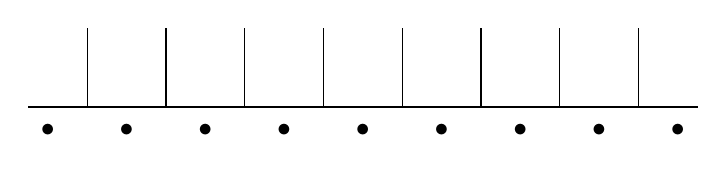
\begin{tikzpicture}
			\draw (-0.25,0) -- (8.25,0);
			\draw (0.5,0) -- (0.5,1);
			\draw (1.5,0) -- (1.5,1);
			\draw (2.5,0) -- (2.5,1);
			\draw (3.5,0) -- (3.5,1);
			\draw (4.5,0) -- (4.5,1);
			\draw (5.5,0) -- (5.5,1);
			\draw (6.5,0) -- (6.5,1);
			\draw (7.5,0) -- (7.5,1);
			\node at (0,-0.3) {$\bullet$};
			\node at (1,-0.3) {$\bullet$};
			\node at (2,-0.3) {$\bullet$};
			\node at (3,-0.3) {$\bullet$};
			\node at (4,-0.3) {$\bullet$};
			\node at (5,-0.3) {$\bullet$};
			\node at (6,-0.3) {$\bullet$};
			\node at (7,-0.3) {$\bullet$};
			\node at (8,-0.3) {$\bullet$};
		\end{tikzpicture}
	\end{figure}
\noindent
where the vertical lines are fixed and the bullets can either be $0$ or $1$ (according to the fusion rules), hence each bullet represents the space $\mathbb{C}^2$.
If we, for instance, only fuse $1$-particles to the chain, the value of the bullets is fixed by the fusion rules: When we fix the boundary labels (e.g., to $1$), the only possible labelling is
	\begin{figure}[H]
		\begin{tikzpicture}
			\draw (-0.25,0) -- (8.25,0);
			\draw (0.5,0) -- (0.5,1);
			\draw (1.5,0) -- (1.5,1);
			\draw (2.5,0) -- (2.5,1);
			\draw (3.5,0) -- (3.5,1);
			\draw (4.5,0) -- (4.5,1);
			\draw (5.5,0) -- (5.5,1);
			\draw (6.5,0) -- (6.5,1);
			\draw (7.5,0) -- (7.5,1);
			\node at (0.5,1.3) {$1$};
			\node at (1.5,1.3) {$1$};
			\node at (2.5,1.3) {$1$};
			\node at (3.5,1.3) {$1$};
			\node at (4.5,1.3) {$1$};
			\node at (5.5,1.3) {$1$};
			\node at (6.5,1.3) {$1$};
			\node at (7.5,1.3) {$1$};
			\node at (0,-0.3) {$1$};
			\node at (1,-0.3) {$0$};
			\node at (2,-0.3) {$1$};
			\node at (3,-0.3) {$0$};
			\node at (4,-0.3) {$1$};
			\node at (5,-0.3) {$0$};
			\node at (6,-0.3) {$1$};
			\node at (7,-0.3) {$0$};
			\node at (8,-0.3) {$1$};
		\end{tikzpicture}
	\end{figure}
\noindent
Hence, we have a unique ground state and the only vertices occurring in this case are
	\begin{figure}[H]	
		\begin{tikzpicture}
			\draw (0,0) -- (1.5,0);
			\draw (0.75,0) -- (0.75,1);
			\node at (0,-0.3) {$0$};
			\node at (1.5,-0.3) {$1$};
			\node at (0.75,1.3) {$1$};
		\end{tikzpicture}
		\hspace{20pt}
		\begin{tikzpicture}
			\draw (0,0) -- (1.5,0);
			\draw (0.75,0) -- (0.75,1);
			\node at (0,-0.3) {$1$};
			\node at (1.5,-0.3) {$0$};
			\node at (0.75,1.3) {$1$};
		\end{tikzpicture}
	\end{figure}
\noindent
Analogously, if we only allow $0$s to fuse to the chain, and the outer labels are fixed to $1$, the only possible labeling is 
	\begin{figure}[H]
		\begin{tikzpicture}
		\draw (-0.25,0) -- (8.25,0);
		\draw (0.5,0) -- (0.5,1);
		\draw (1.5,0) -- (1.5,1);
		\draw (2.5,0) -- (2.5,1);
		\draw (3.5,0) -- (3.5,1);
		\draw (4.5,0) -- (4.5,1);
		\draw (5.5,0) -- (5.5,1);
		\draw (6.5,0) -- (6.5,1);
		\draw (7.5,0) -- (7.5,1);
		\node at (0.5,1.3) {$0$};
		\node at (1.5,1.3) {$0$};
		\node at (2.5,1.3) {$0$};
		\node at (3.5,1.3) {$0$};
		\node at (4.5,1.3) {$0$};
		\node at (5.5,1.3) {$0$};
		\node at (6.5,1.3) {$0$};
		\node at (7.5,1.3) {$0$};
		\node at (0,-0.3) {$1$};
		\node at (1,-0.3) {$1$};
		\node at (2,-0.3) {$1$};
		\node at (3,-0.3) {$1$};
		\node at (4,-0.3) {$1$};
		\node at (5,-0.3) {$1$};
		\node at (6,-0.3) {$1$};
		\node at (7,-0.3) {$1$};
		\node at (8,-0.3) {$1$};
		\end{tikzpicture}
	\end{figure}
	\noindent
If we had fixed the outer labels to $0$, all bullets would have to be $0$. Hence, the only vertices occurring in these cases are
	\begin{figure}[H]	
		\begin{tikzpicture}
		\draw (0,0) -- (1.5,0);
		\draw (0.75,0) -- (0.75,1);
		\node at (0,-0.3) {$0$};
		\node at (1.5,-0.3) {$0$};
		\node at (0.75,1.3) {$0$};
		\end{tikzpicture}
		\hspace{20pt}
		\begin{tikzpicture}
		\draw (0,0) -- (1.5,0);
		\draw (0.75,0) -- (0.75,1);
		\node at (0,-0.3) {$1$};
		\node at (1.5,-0.3) {$1$};
		\node at (0.75,1.3) {$0$};
		\end{tikzpicture}
	\end{figure}
\noindent
This means that in the case of open boundary conditions, the chain has a \emph{unique ground state} once we fix the outer labels of the chain. The situation is different for periodic boundary conditions: since the only requirement here is that the label at site $n+1$ has to equal the label at site $1$, there are always two possibilities of labeling the chain. For instance, in the case of only fusing $1$s to the chain, the two possibilities are
	\begin{figure}[H]
		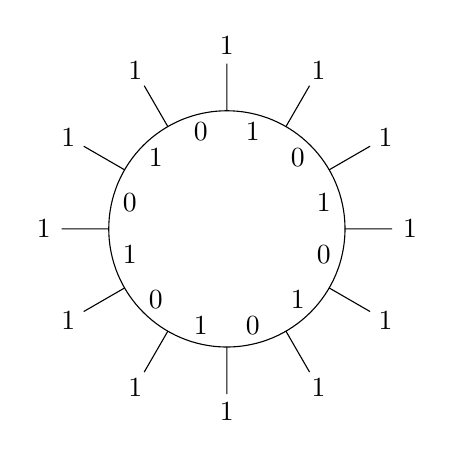
\begin{tikzpicture}[scale=1.5]
			\def\Radius{1cm}
			\draw (0,0) circle[radius=\Radius];
			\draw
			\foreach \a in {0, 30, ..., 330} {
				(\a:\Radius) -- (\a:1.4)
			};
			\foreach \a in {0, 30, ..., 330} {
				\node at (\a:1.55) {$1$};
			};
			\foreach \a in {45, 105, ..., 375} {
				\node at (\a:0.85) {$0$};
			};
			\foreach \a in {15, 75, ..., 315} {
				\node at (\a:0.85) {$1$};
			};
		\end{tikzpicture}
		\hspace{40pt}
		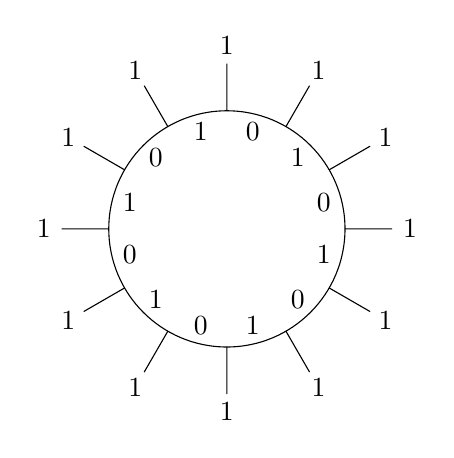
\begin{tikzpicture}[scale=1.5]
			\def\Radius{1cm}
			\draw (0,0) circle[radius=\Radius];
			\draw
			\foreach \a in {0, 30, ..., 330} {
				(\a:\Radius) -- (\a:1.4)
			};
			\foreach \a in {0, 30, ..., 330} {
				\node at (\a:1.55) {$1$};
			};
			\foreach \a in {45, 105, ..., 375} {
				\node at (\a:0.85) {$1$};
			};
			\foreach \a in {15, 75, ..., 315} {
				\node at (\a:0.85) {$0$};
			};
		\end{tikzpicture}
	\end{figure}
\noindent
In case of fusing $0$ to the chain, we can either allow only $0$s or only $1$ as labels of the chain. Therefore, the chain with periodic boundary conditions has two ground states, hence it represents a qubit.

We will now introduce defects to this model, indicated by red lines that fuse to the chain, e.g.\ a chain with one defect would be
	\begin{figure}[H]
		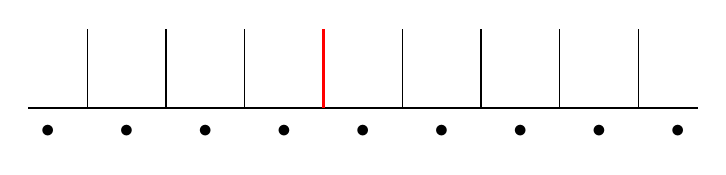
\begin{tikzpicture}
		\draw (-0.25,0) -- (8.25,0);
		\draw (0.5,0) -- (0.5,1);
		\draw (1.5,0) -- (1.5,1);
		\draw (2.5,0) -- (2.5,1);
		\draw[red,line width=0.4mm] (3.5,0) -- (3.5,1);
		\draw (4.5,0) -- (4.5,1);
		\draw (5.5,0) -- (5.5,1);
		\draw (6.5,0) -- (6.5,1);
		\draw (7.5,0) -- (7.5,1);
		\node at (0,-0.3) {$\bullet$};
		\node at (1,-0.3) {$\bullet$};
		\node at (2,-0.3) {$\bullet$};
		\node at (3,-0.3) {$\bullet$};
		\node at (4,-0.3) {$\bullet$};
		\node at (5,-0.3) {$\bullet$};
		\node at (6,-0.3) {$\bullet$};
		\node at (7,-0.3) {$\bullet$};
		\node at (8,-0.3) {$\bullet$};
		\end{tikzpicture}
	\end{figure}
	\noindent
Since the chain is represented by a category, $\Vec(\Z/2\Z)$ in our example, the defect is a $\Vec(\Z/2\Z)-\Vec(\Z/2\Z)$ bimodule, i.e.\ we are fusing an object from the bimodule to the chain. Here, we will use the bimodule $F_1$ to introduce defects to the $\Vec(\Z/2\Z)$-chain. $F_1$ has only one object, so in general we omit writing labels for the bimodule object, but indicate by a red line when the object is from the bimodule. When it is inevitable to indicate the label, we denote it $*$.

The occurrence of one defect in a chain does not change the ground state of the system; The labels on the chain are still determined by the choice of labels on the boundary. This is different if we have more than one defect in the chain. For instance, for two defects the chain is
	\begin{figure}[H]
		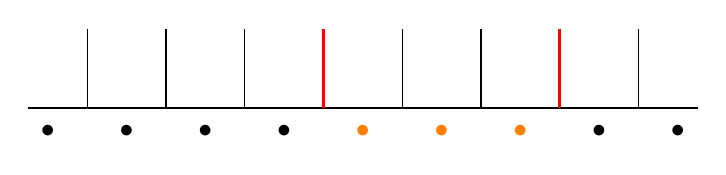
\begin{tikzpicture}
		\draw (-0.25,0) -- (8.25,0);
		\draw (0.5,0) -- (0.5,1);
		\draw (1.5,0) -- (1.5,1);
		\draw (2.5,0) -- (2.5,1);
		\draw[red,line width=0.4mm] (3.5,0) -- (3.5,1);
		\draw (4.5,0) -- (4.5,1);
		\draw (5.5,0) -- (5.5,1);
		\draw[red,line width=0.4mm] (6.5,0) -- (6.5,1);
		\draw (7.5,0) -- (7.5,1);
		\node at (0,-0.3) {$\bullet$};
		\node at (1,-0.3) {$\bullet$};
		\node at (2,-0.3) {$\bullet$};
		\node at (3,-0.3) {$\bullet$};
		\node at (4,-0.3) {{\color{orange}$\bullet$}};
		\node at (5,-0.3) {{\color{orange}$\bullet$}};
		\node at (6,-0.3) {{\color{orange}$\bullet$}};
		\node at (7,-0.3) {$\bullet$};
		\node at (8,-0.3) {$\bullet$};
		\end{tikzpicture}
	\end{figure}
\noindent
where the colour of the orange bullets is not determined by the labels on the boundary of the chain. Hence, we get an additional qubit. In general, the number of additional qubits in the chain is $\#\mathrm{defects}-1$. This can be done analogously for the chain with periodic boundary conditions, the only difference is that in this case, we already have one qubit when there is no defect. By introducing defects to the chain, we have also introduced a new vertex to our model
	\begin{figure}[H]	
		\begin{tikzpicture}
		\draw[red] (0,0) -- (1.5,0);
		\draw[black,line width=0.4mm] (0.75,0) -- (0.75,1);
		\end{tikzpicture}
	\end{figure}
\noindent
where any object from $\Vec(\Z/2\Z)$ can be on the black line. Since this vertex is neither defined in the category $\Vec(\Z/2\Z)$ nor in the bimodule $F_1$, we need to construct it. More precisely, for each choice of labels we need a basis for the corresponding morphism space. We could also allow the bimodule object to live on the horizontal lines of the chain, which would require the construction of additional vertices. 
%For now, we will restrict to the case that only objects of the category are allowed to be on horizontal lines, but we will come back to other possibilities later. Although we will not need this specific vertex in the final chain we are going to construct, we go through its computation in detail to explain how these vertices can be constructed in general. 
We do the construction of the required vertex step-by-step in the following by using ideas from tube algebras. 

\subsection*{Step 1: Compute isomorphism classes of objects and pick a representative} In general, what we aim for are representations of the tube algebra of the form
	\begin{figure}[H]
		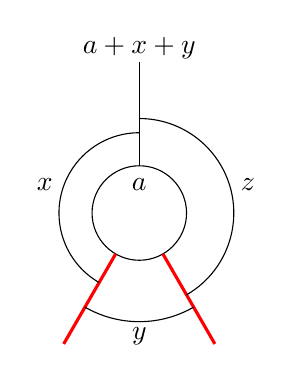
\begin{tikzpicture}[scale=1.2]
			\draw (0,0) circle (0.5cm);
			\draw[red,line width=0.4mm]
			\foreach \a in {-60, -120} {
				(\a:0.5) -- (\a:1.6)
			};
			\draw ([shift=(-60:1cm)]0,0) arc (-60:90:1cm);
			\draw ([shift=(-120:1.15cm)]0,0) arc (-120:-60:1.15cm);
			\draw ([shift=(240:0.85cm)]0,0) arc (240:90:0.85cm);
			\draw[] (90:0.5) -- (90:1.6);
			\node at (90:.3cm){$a$};\node at (90:1.75cm){$a+x+y$};
			\node at (-1,0.3) {$x$};
			\node at (1.15,0.3) {$z$};
			\node at (0,-1.3) {$y$};
		\end{tikzpicture}
	\end{figure}
\noindent
According to the figure above, $(*,*,a)\cong(*,*,a+x+y)$ for all possible labels $x,y,z$, so we pick $(*,*,0)$ as a representative.

\subsection{Step 2: Find primitive idempotents} To find a representation of the tube algebra, we need to compute the primitive idempotents, i.e. we need to find morphisms that map $(*,*,0)$ to $(*,*,0)$ which square to themselves and are orthogonal to each other. Additionally, since we want \emph{primitive} idempotents, we need to make sure that they cannot be written as the sum of idempotents.
Candidates for idempotents are the morphism where $x+y=0$:
	\begin{equation}
		T_{0,0}=
		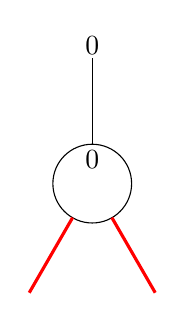
\begin{tikzpicture}[scale=1,baseline=(current bounding box.center)]
			\draw (0,0) circle (0.5cm);
			\draw[red,line width=0.4mm]
			\foreach \a in {-60, -120} {
				(\a:0.5) -- (\a:1.6)
			};
%			\draw ([shift=(-60:1cm)]0,0) arc (-60:90:1cm);
%			\draw ([shift=(-120:1.15cm)]0,0) arc (-120:-60:1.15cm);
%			\draw ([shift=(240:0.85cm)]0,0) arc (240:90:0.85cm);
			\draw[] (90:0.5) -- (90:1.6);
			\node at (90:.3cm){$0$};\node at (90:1.75cm){$0$};
%			\node at (-1,0.3) {$0$};
%			\node at (1.15,0.3) {$0$};
%			\node at (0,-1.3) {$0$};
		\end{tikzpicture}
		\hspace{5mm}
		T_{0,1}:=
		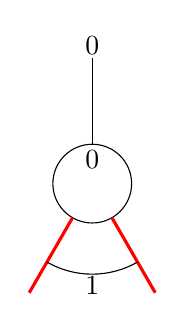
\begin{tikzpicture}[scale=1,baseline=(current bounding box.center)]
		\draw (0,0) circle (0.5cm);
		\draw[red,line width=0.4mm]
		\foreach \a in {-60, -120} {
			(\a:0.5) -- (\a:1.6)
		};
%		\draw ([shift=(-60:1cm)]0,0) arc (-60:90:1cm);
		\draw ([shift=(-120:1.15cm)]0,0) arc (-120:-60:1.15cm);
%		\draw ([shift=(240:0.85cm)]0,0) arc (240:90:0.85cm);
		\draw[] (90:0.5) -- (90:1.6);
		\node at (90:.3cm){$0$};\node at (90:1.75cm){$0$};
%		\node at (-1,0.3) {$0$};
%		\node at (1.15,0.3) {$0$};
		\node at (0,-1.3) {$1$};
		\end{tikzpicture}
		\hspace{5mm}
		T_{1,0}:=
		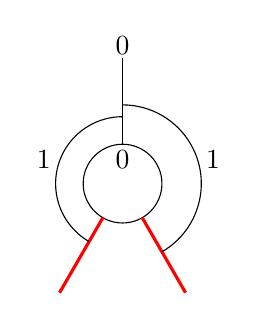
\begin{tikzpicture}[scale=1,baseline=(current bounding box.center)]
		\draw (0,0) circle (0.5cm);
		\draw[red,line width=0.4mm]
		\foreach \a in {-60, -120} {
			(\a:0.5) -- (\a:1.6)
		};
		\draw ([shift=(-60:1cm)]0,0) arc (-60:90:1cm);
%		\draw ([shift=(-120:1.15cm)]0,0) arc (-120:-60:1.15cm);
		\draw ([shift=(240:0.85cm)]0,0) arc (240:90:0.85cm);
		\draw[] (90:0.5) -- (90:1.6);
		\node at (90:.3cm){$0$};\node at (90:1.75cm){$0$};
		\node at (-1,0.3) {$1$};
		\node at (1.15,0.3) {$1$};
%		\node at (0,-1.3) {$0$};
		\end{tikzpicture}
		\hspace{5mm}
		T_{1,1}:=
		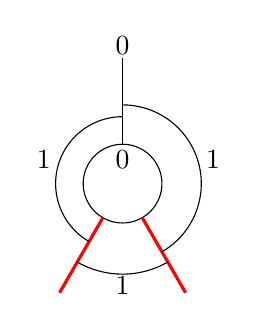
\begin{tikzpicture}[scale=1,baseline=(current bounding box.center)]
		\draw (0,0) circle (0.5cm);
		\draw[red,line width=0.4mm]
		\foreach \a in {-60, -120} {
			(\a:0.5) -- (\a:1.6)
		};
		\draw ([shift=(-60:1cm)]0,0) arc (-60:90:1cm);
		\draw ([shift=(-120:1.15cm)]0,0) arc (-120:-60:1.15cm);
		\draw ([shift=(240:0.85cm)]0,0) arc (240:90:0.85cm);
		\draw[] (90:0.5) -- (90:1.6);
		\node at (90:.3cm){$0$};\node at (90:1.75cm){$0$};
		\node at (-1,0.3) {$1$};
		\node at (1.15,0.3) {$1$};
		\node at (0,-1.3) {$1$};
		\end{tikzpicture}
	\end{equation}
\noindent
The first morphism can be interpreted as the identity morphism and it obviously squares to itself. It is easy to see that the second and third diagrams square to the first. To square the final morphism, we need to do the following calculation:\vspace{5pt}
	\begin{equation*}
		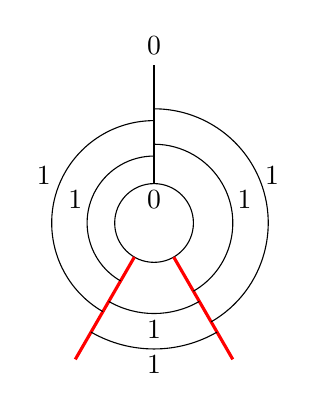
\begin{tikzpicture}[scale=1,baseline=(current bounding box.center)]
			\draw (0,0) circle (0.5cm);
			\draw[red,line width=0.4mm]
			\foreach \a in {-60, -120} {
				(\a:0.5) -- (\a:2)
			};
			\draw[] (90:0.5) -- (90:2);
			\draw ([shift=(-60:1cm)]0,0) arc (-60:90:1cm);
			\draw ([shift=(-120:1.15cm)]0,0) arc (-120:-60:1.15cm);
			\draw ([shift=(240:0.85cm)]0,0) arc (240:90:0.85cm);
			\draw ([shift=(240:1.3cm)]0,0) arc (240:90:1.3cm);
			\draw ([shift=(-60:1.45cm)]0,0) arc (-60:90:1.45cm);
			\draw ([shift=(-120:1.6cm)]0,0) arc (-120:-60:1.6cm);
			\node at (90:.3cm){$0$};\node at (90:2.25cm){$0$};
			\node at (-1,0.3) {$1$};
			\node at (1.15,0.3) {$1$};
			\node at (0,-1.35) {$1$};
			\node at (-1.4,0.6) {$1$};
			\node at (1.5,0.6) {$1$};
			\node at (0,-1.8) {$1$};
		\end{tikzpicture}
		=-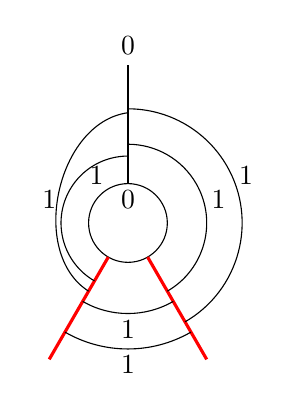
\begin{tikzpicture}[scale=1,baseline=(current bounding box.center)]
			\draw (0,0) circle (0.5cm);
			\draw[red,line width=0.4mm]
			\foreach \a in {-60, -120} {
				(\a:0.5) -- (\a:2)
			};
			\draw[] (90:0.5) -- (90:2);
			\draw ([shift=(-60:1cm)]0,0) arc (-60:90:1cm);
			\draw ([shift=(-120:1.15cm)]0,0) arc (-120:-60:1.15cm);
			\draw ([shift=(240:0.85cm)]0,0) arc (240:90:0.85cm);
%			\draw ([shift=(240:1.3cm)]0,0) arc (240:90:1.3cm);
			\draw[] ([shift=(240:1.0cm)]0,0) to [bend left=70] ([shift=(90:1.4cm)]0,0);
			\draw ([shift=(-60:1.45cm)]0,0) arc (-60:90:1.45cm);
			\draw ([shift=(-120:1.6cm)]0,0) arc (-120:-60:1.6cm);
			\node at (90:.3cm){$0$};\node at (90:2.25cm){$0$};
			\node at (-1,0.3) {$1$};
			\node at (1.15,0.3) {$1$};
			\node at (0,-1.35) {$1$};
			\node at (-.4,0.6) {$1$};
			\node at (1.5,0.6) {$1$};
			\node at (0,-1.8) {$1$};
		\end{tikzpicture}
		=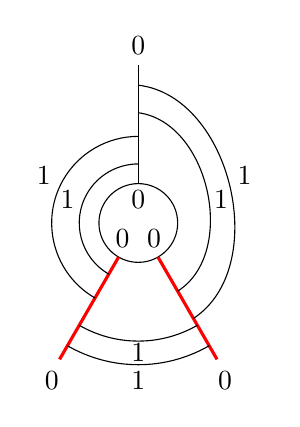
\begin{tikzpicture}[scale=1,baseline=(current bounding box.center)]
			\draw (0,0) circle (0.5cm);
			\draw[red,line width=0.4mm]
			\foreach \a in {-60, -120} {
				(\a:0.5) -- (\a:2)
			};
			\draw[] (90:0.5) -- (90:2);
			\draw ([shift=(240:0.75cm)]0,0) arc (240:90:0.75cm);
			%\draw ([shift=(-60:1.2cm)]0,0) arc (-60:90:1.2cm);
			\draw ([shift=(-60:1cm)]0,0) to [bend right=70] ([shift=(90:1.4cm)]0,0);
			\draw ([shift=(-120:1.5cm)]0,0) arc (-120:-60:1.5cm);
			\draw ([shift=(240:1.1cm)]0,0) arc (240:90:1.1cm);
			%\draw ([shift=(-60:1.6cm)]0,0.2) arc (-60:90:1.6cm);
			\draw ([shift=(-60:1.4cm)]0,0) to [bend right=70] ([shift=(90:1.75cm)]0,0);
			\draw ([shift=(-120:1.8cm)]0,0) arc (-120:-60:1.8cm);
			\node at (90:.3cm){$0$};\node at (90:2.25cm){$0$};
			\node at (0.2,-0.2) {$0$};
			\node at (-0.2,-0.2) {$0$};
			\node at (-1.1,-2) {$0$};
			\node at (1.1,-2) {$0$};
			\node at (-0.9,0.3) {$1$};
			\node at (1.05,0.3) {$1$};
			\node at (0,-1.65) {$1$};
			\node at (-1.2,0.6) {$1$};
			\node at (1.35,0.6) {$1$};
			\node at (0,-2) {$1$};
		\end{tikzpicture}
		=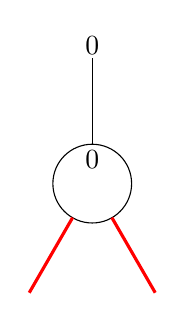
\begin{tikzpicture}[scale=1,baseline=(current bounding box.center)]
			\draw (0,0) circle (0.5cm);
			\draw[red,line width=0.4mm]
			\foreach \a in {-60, -120} {
				(\a:0.5) -- (\a:1.6)
			};
			\draw[] (90:0.5) -- (90:1.6);
			\node at (90:.3cm){$0$};\node at (90:1.75cm){$0$};
%			\draw ([shift=(-60:1cm)]0,0) arc (-60:90:1cm);
%			\draw ([shift=(-120:1.15cm)]0,0) arc (-120:-60:1.15cm);
%			\draw ([shift=(240:0.85cm)]0,0) arc (240:90:0.85cm);
%			\node at (0.2,-0.2) {$0$};
%			\node at (-0.2,-0.2) {$0$};
%			\node at (-0.9,-1.6) {$0$};
%			\node at (0.9,-1.6) {$0$};
%			\node at (-1,0.3) {$0$};
%			\node at (1.15,0.3) {$0$};
%			\node at (0,-1.35) {$0$};
		\end{tikzpicture}\vspace{5pt}
	\end{equation*}
Hence, the second candidate does not square to itself but to the first candidate. 
Similar computations show that $T_{a,b}T_{c,d}=T_{a+c,b+d}$. 
However, since the primitive idempotents form an algebra, we can also consider linear combinations of the candidates. Also, because we have four candidates, we know that the algebra is $4$-dimensional. To find out the primitive idempotents from the candidates, it is convenient to find a representation of them in terms of matrices, i.e.\ we need matrices that multiply in the same way as the candidates. As mentioned above, the first candidate is the identity, hence the corresponding matrix is
	\begin{equation}
		M_{0,0}=\begin{pmatrix}
			1 & 0 & 0 & 0\\
			0 & 1 & 0 & 0\\
			0 & 0 & 1 & 0\\
			0 & 0 & 0 & 1\\
		\end{pmatrix}.
	\end{equation}
From this representation it is clear that this candidate is an idempotent, but not a primitive one: $M_{0,0}$ can be written as
	\begin{equation}
	\label{eq_M0}
		M_{0,0}=
		\begin{pmatrix}
		1 & 0 & 0 & 0\\
		0 & 0 & 0 & 0\\
		0 & 0 & 0 & 0\\
		0 & 0 & 0 & 0\\
		\end{pmatrix}
		+\begin{pmatrix}
		0 & 0 & 0 & 0\\
		0 & 1 & 0 & 0\\
		0 & 0 & 0 & 0\\
		0 & 0 & 0 & 0\\
		\end{pmatrix}
		+
		\begin{pmatrix}
		0 & 0 & 0 & 0\\
		0 & 0 & 0 & 0\\
		0 & 0 & 1 & 0\\
		0 & 0 & 0 & 0\\
		\end{pmatrix}
		+\begin{pmatrix}
		0 & 0 & 0 & 0\\
		0 & 0 & 0 & 0\\
		0 & 0 & 0 & 0\\
		0 & 0 & 0 & 1\\
		\end{pmatrix}
		.
	\end{equation}
The matrix representing the second candidate has to fulfill $M_{0,1}^2=M_{0,0}$, so a possible choice is
	\begin{equation}
		M_{0,1}=\begin{pmatrix}
			1 & 0 & 0 & 0\\
			0 & 1 & 0 & 0\\
			0 & 0 & -1 & 0\\
			0 & 0 & 0 & -1\\
		\end{pmatrix}.
	\end{equation}
	Similar matrices can be found for the remaining morphisms.
From \eqref{eq_M0}, we get four candidates for primitive idempotents. They are indeed primitive idempotents in the algebra of $4$-dimensional matrices. To translate them back into annular diagrams, we just need to express them in terms of $M_{a,b}$, which yields
	\begin{align}
	P_{x,y}=\frac{1}{4}\sum_{a,b}(-1)^{ax+by}M_{a,b}
	\end{align}
which is diagrammatically
	\begin{equation}
		P_{x,y}=\frac{1}{4}\left(
			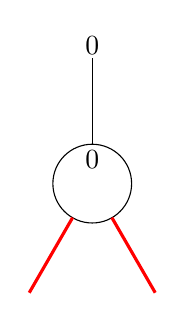
\begin{tikzpicture}[scale=1,baseline=(current bounding box.center)]
			\draw (0,0) circle (0.5cm);
			\draw[red,line width=0.4mm]
			\foreach \a in {-60, -120} {
				(\a:0.5) -- (\a:1.6)
			};
			%			\draw ([shift=(-60:1cm)]0,0) arc (-60:90:1cm);
			%			\draw ([shift=(-120:1.15cm)]0,0) arc (-120:-60:1.15cm);
			%			\draw ([shift=(240:0.85cm)]0,0) arc (240:90:0.85cm);
			\draw[] (90:0.5) -- (90:1.6);
			\node at (90:.3cm){$0$};\node at (90:1.75cm){$0$};
			%			\node at (-1,0.3) {$0$};
			%			\node at (1.15,0.3) {$0$};
			%			\node at (0,-1.3) {$0$};
			\end{tikzpicture}
			(-1)^x
			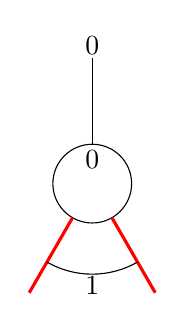
\begin{tikzpicture}[scale=1,baseline=(current bounding box.center)]
			\draw (0,0) circle (0.5cm);
			\draw[red,line width=0.4mm]
			\foreach \a in {-60, -120} {
				(\a:0.5) -- (\a:1.6)
			};
%						\draw ([shift=(-60:1cm)]0,0) arc (-60:90:1cm);
			\draw ([shift=(-120:1.15cm)]0,0) arc (-120:-60:1.15cm);
%						\draw ([shift=(240:0.85cm)]0,0) arc (240:90:0.85cm);
			\draw[] (90:0.5) -- (90:1.6);
			\node at (90:.3cm){$0$};\node at (90:1.75cm){$0$};
			%			\node at (-1,0.3) {$0$};
%						\node at (1.15,0.3) {$0$};
						\node at (0,-1.3) {$1$};
			\end{tikzpicture}
			(-1)^y
			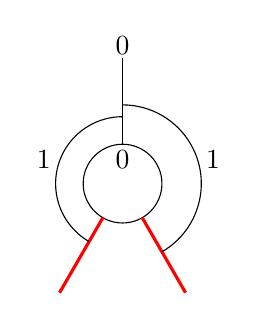
\begin{tikzpicture}[scale=1,baseline=(current bounding box.center)]
			\draw (0,0) circle (0.5cm);
			\draw[red,line width=0.4mm]
			\foreach \a in {-60, -120} {
				(\a:0.5) -- (\a:1.6)
			};
									\draw ([shift=(-60:1cm)]0,0) arc (-60:90:1cm);
%			\draw ([shift=(-120:1.15cm)]0,0) arc (-120:-60:1.15cm);
									\draw ([shift=(240:0.85cm)]0,0) arc (240:90:0.85cm);
			\draw[] (90:0.5) -- (90:1.6);
			\node at (90:.3cm){$0$};\node at (90:1.75cm){$0$};
						\node at (-1,0.3) {$1$};
									\node at (1.15,0.3) {$1$};
%			\node at (0,-1.3) {$1$};
			\end{tikzpicture}
			(-1)^{x+y}
			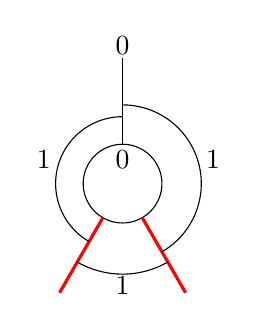
\begin{tikzpicture}[scale=1,baseline=(current bounding box.center)]
			\draw (0,0) circle (0.5cm);
			\draw[red,line width=0.4mm]
			\foreach \a in {-60, -120} {
				(\a:0.5) -- (\a:1.6)
			};
									\draw ([shift=(-60:1cm)]0,0) arc (-60:90:1cm);
			\draw ([shift=(-120:1.15cm)]0,0) arc (-120:-60:1.15cm);
									\draw ([shift=(240:0.85cm)]0,0) arc (240:90:0.85cm);
			\draw[] (90:0.5) -- (90:1.6);
			\node at (90:.3cm){$0$};\node at (90:1.75cm){$0$};
			\node at (-1,0.3) {$1$};
			\node at (1.15,0.3) {$1$};
			\node at (0,-1.3) {$1$};
			\end{tikzpicture}
			\right).
	\end{equation}
	
\subsection*{Step 3: Check for isomorphism classes of primitive idempotents} In general, it is possible that the primitive idempotents we just found are isomorphic to each other, which means that there are matrices within the algebra that we can multiply to $P_{0,0}$, for example, and get $P_{1,0}$. The following equation is an example for how this works:
	\begin{equation}
		\begin{pmatrix} 0 & 0 & 0 & 0\\ 1 & 0 & 0 & 0\\ 0 & 0 & 0 & 0\\ 0 & 0 & 0 & 0\\ \end{pmatrix}P_{0,0} \begin{pmatrix} 0 & 1 & 0 & 0\\ 0 & 0 & 0 & 0\\ 0 & 0 & 0 & 0\\ 0 & 0 & 0 & 0\\ \end{pmatrix}=P_{1,0}.\label{eqn:isoids}
	\end{equation}
However, the two matrices we multiply $P_{0,0}$ with are not elements of the matrix algebra (the matrices on the algebra only have entries on the diagonal). If they were elements of the algebra, they would form an isomorphism between $P_{0,0}$ and $P_{1,0}$, so we would pick one of them as a representative.

This step can be much more complicated for algebras with bigger dimensions. However, there is a nice trick which helps to see how many isomorphism classes there are, which is the Artin-Wedderburn theorem. It states that any semi-simple algebra can be decomposed into a direct sum of full matrix algebras, i.e.
	\begin{equation}
		\mathcal{M}\cong\bigoplus\mathcal{M}_d,
	\end{equation}
	where $\dim{\mathcal{M}_d}=d^2$. Within a full matrix algebra we can pick, for example, the primitive idempotent $\mathrm{diag}(1,0,\ldots)$ since the equivalent of the matrices in Eqn.~\ref{eqn:isoids} exist. We therefore only get one primitive idempotent for each full matrix algebra. In our example, the algebra is 4 dimensional. The possible decompositions are therefore 
	$\mathcal{M}\cong\mathbb{C}\oplus\mathbb{C}\oplus\mathbb{C}\oplus\mathbb{C}$ and $\mathcal{M}_2$. We found the first decomposition was correct so we get four primitive idempotents (as we showed above). 
	In case of a $5$-dimensional matrix algebra, the possible decompositions are
	\begin{equation}
		\mathcal{M}_{5-\mathrm{dim}}\cong\mathbb{C}\oplus\mathcal{M}_2(\mathbb{C}),
	\end{equation}
	or 
	\begin{equation}
		\mathcal{M}_{5-\mathrm{dim}}\cong5\mathbb{C},
	\end{equation}
so we get two or five primitive idempotents respectively.
	
\subsection*{Step 4: Build the full representation} After we have found the primitive idempotents of the algebra, we can build the full representation. This is done by putting all possible tubes on the outside of the idempotents, hence finding all the basis vectors for this space, i.e.\ all possible vectors
	\begin{equation}
		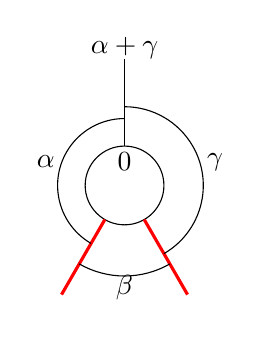
\begin{tikzpicture}[scale=1,baseline=(current bounding box.center)]
		\draw (0,0) circle (0.5cm);
		\draw[red,line width=0.4mm]
		\foreach \a in {-60, -120} {
			(\a:0.5) -- (\a:1.6)
		};
		\draw ([shift=(-60:1cm)]0,0) arc (-60:90:1cm);
		\draw ([shift=(-120:1.15cm)]0,0) arc (-120:-60:1.15cm);
		\draw ([shift=(240:0.85cm)]0,0) arc (240:90:0.85cm);
		\draw[] (90:0.5) -- (90:1.6);
		\node at (90:.3cm){$0$};\node at (90:1.75cm){$\alpha+\gamma$};
		\node at (-1,0.3) {$\alpha$};
		\node at (1.15,0.3) {$\gamma$};
		\node at (0,-1.3) {$\beta$};
		\end{tikzpicture}
	\end{equation}
%\noindent
In general, the basis vectors are determined by the choice of $\alpha,\beta$ and $\gamma$, therefore there are up to $2^3=8$ possible basis vectors for each representation. However, it is possible that some of these vectors are linearly dependent, which is the case in our example, as we will see. Putting the general tubes around the primitive idempotents $P_{x,y}$ yields
	\begin{align}
	\frac{1}{4}
	\sum_{a,b}(-1)^{ax+by}
	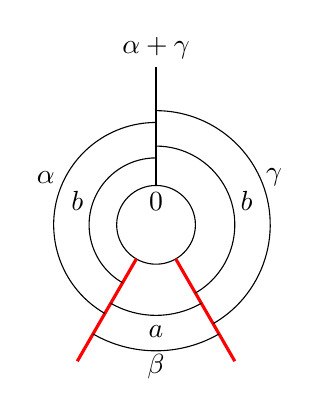
\begin{tikzpicture}[scale=1,baseline=(current bounding box.center)]
	\draw (0,0) circle (0.5cm);
	\draw[red,line width=0.4mm]
	\foreach \a in {-60, -120} {
		(\a:0.5) -- (\a:2)
	};
	\draw[] (90:0.5) -- (90:2);
	\draw ([shift=(-60:1cm)]0,0) arc (-60:90:1cm);
	\draw ([shift=(-120:1.15cm)]0,0) arc (-120:-60:1.15cm);
	\draw ([shift=(240:0.85cm)]0,0) arc (240:90:0.85cm);
	\draw ([shift=(240:1.3cm)]0,0) arc (240:90:1.3cm);
	\draw ([shift=(-60:1.45cm)]0,0) arc (-60:90:1.45cm);
	\draw ([shift=(-120:1.6cm)]0,0) arc (-120:-60:1.6cm);
	\node at (90:.3cm){$0$};\node at (90:2.25cm){$\alpha+\gamma$};
	\node at (-1,0.3) {$b$};
	\node at (1.15,0.3) {$b$};
	\node at (0,-1.35) {$a$};
	\node at (-1.4,0.6) {$\alpha$};
	\node at (1.5,0.6) {$\gamma$};
	\node at (0,-1.8) {$\beta$};
	\end{tikzpicture}
	&=
	\frac{1}{4}
	\sum_{a,b}(-1)^{a(x+\alpha+\gamma)+by}
	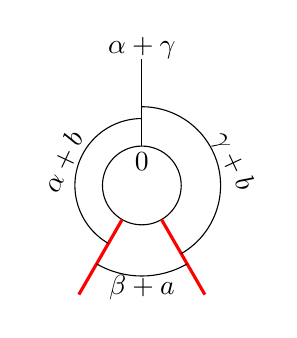
\begin{tikzpicture}[scale=1,baseline=(current bounding box.center)]
	\draw (0,0) circle (0.5cm);
	\draw[red,line width=0.4mm]
	\foreach \a in {-60, -120} {
		(\a:0.5) -- (\a:1.6)
	};
	\draw ([shift=(-60:1cm)]0,0) arc (-60:90:1cm);
	\draw ([shift=(-120:1.15cm)]0,0) arc (-120:-60:1.15cm);
	\draw ([shift=(240:0.85cm)]0,0) arc (240:90:0.85cm);
	\draw[] (90:0.5) -- (90:1.6);
	\node at (90:.3cm){$0$};\node at (90:1.75cm){$\alpha+\gamma$};
	\node[rotate=65] at (-1,0.3) {$\alpha+b$};
	\node[rotate=-65] at (1.15,0.3) {$\gamma+b$};
	\node at (0,-1.3) {$\beta+a$};
	\end{tikzpicture}\\
	&=
	\frac{(-1)^{(x+\alpha^\prime)\beta+y\gamma}}{4}
	\sum_{a^\prime,b^\prime}(-1)^{a^\prime(x+\alpha^\prime)+b^\prime y}
	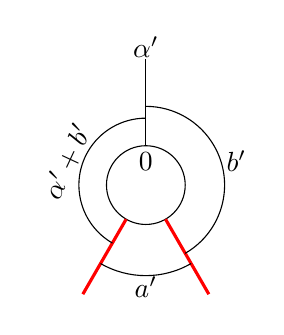
\begin{tikzpicture}[scale=1,baseline=(current bounding box.center)]
	\draw (0,0) circle (0.5cm);
	\draw[red,line width=0.4mm]
	\foreach \a in {-60, -120} {
		(\a:0.5) -- (\a:1.6)
	};
	\draw ([shift=(-60:1cm)]0,0) arc (-60:90:1cm);
	\draw ([shift=(-120:1.15cm)]0,0) arc (-120:-60:1.15cm);
	\draw ([shift=(240:0.85cm)]0,0) arc (240:90:0.85cm);
	\draw[] (90:0.5) -- (90:1.6);
	\node at (90:.3cm){$0$};\node at (90:1.75cm){$\alpha^\prime$};
	\node[rotate=65] at (-1,0.3) {$\alpha^\prime+b^\prime$};
	\node at (1.15,0.3) {$b^\prime$};
	\node at (0,-1.3) {$a^\prime$};
	\end{tikzpicture}
	\end{align}
which is a vector in the morphism space
	\begin{equation}	
		\begin{tikzpicture}
			\draw[red,line width=0.4mm] (0,0) -- (1.5,0);
			\draw (0.75,0) -- (0.75,1) node [pos=1.25]{$\alpha^\prime$};
		\end{tikzpicture}
	\end{equation}
We now have to find a basis for every one of those morphism spaces, i.e.\ for every choice of $\alpha^\prime$. For fixed representation (fixed, $x,y$), we find a unique vector up to a multiplicative scalar for each $\alpha^\prime$, so each morphism space is one dimensional. We define the basis to be
	\begin{equation}
		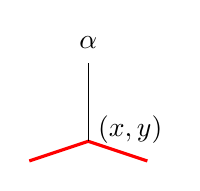
\begin{tikzpicture}[scale=1,baseline=(current bounding box.center)]
			\draw[red,line width=0.4mm] (0,-.25) -- (.75,0) -- (1.5,-.25);
			\draw (0.75,0) -- (0.75,1) node [pos=1.25] {$\alpha$};
			\node[above,right] at (.75,.15) {$(x,y)$};
		\end{tikzpicture}\equiv
		\frac{1}{4}
		\sum_{a^\prime,b^\prime}(-1)^{a(x+\alpha)+b y}
		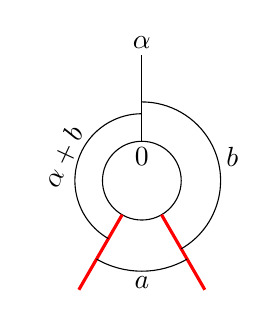
\begin{tikzpicture}[scale=1,baseline=(current bounding box.center)]
		\draw (0,0) circle (0.5cm);
		\draw[red,line width=0.4mm]
		\foreach \a in {-60, -120} {
			(\a:0.5) -- (\a:1.6)
		};
		\draw ([shift=(-60:1cm)]0,0) arc (-60:90:1cm);
		\draw ([shift=(-120:1.15cm)]0,0) arc (-120:-60:1.15cm);
		\draw ([shift=(240:0.85cm)]0,0) arc (240:90:0.85cm);
		\draw[] (90:0.5) -- (90:1.6);
		\node at (90:.3cm){$0$};\node at (90:1.75cm){$\alpha$};
		\node[rotate=65] at (-1,0.3) {$\alpha+b$};
		\node at (1.15,0.3) {$b$};
		\node at (0,-1.3) {$a$};
		\end{tikzpicture}
	\end{equation}
The `inflation trick' developed in Refs.~\cite{BBJ18,BB19a,BB19b} picks out the representation $P_{0,0}$, and we will work with that from here on. This means
	\begin{equation}
	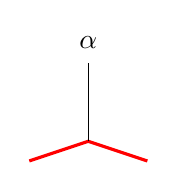
\begin{tikzpicture}[scale=1,baseline=(current bounding box.center)]
	\draw[red,line width=0.4mm] (0,-.25) -- (.75,0) -- (1.5,-.25);
	\draw (0.75,0) -- (0.75,1) node [pos=1.25] {$\alpha$};
	\end{tikzpicture}:=
	\frac{1}{4}
	\sum_{a^\prime,b^\prime}(-1)^{a\alpha}
	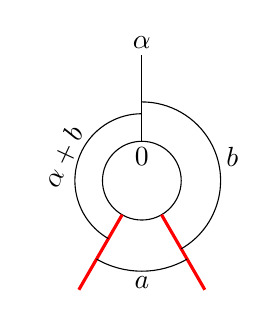
\begin{tikzpicture}[scale=1,baseline=(current bounding box.center)]
	\draw (0,0) circle (0.5cm);
	\draw[red,line width=0.4mm]
	\foreach \a in {-60, -120} {
		(\a:0.5) -- (\a:1.6)
	};
	\draw ([shift=(-60:1cm)]0,0) arc (-60:90:1cm);
	\draw ([shift=(-120:1.15cm)]0,0) arc (-120:-60:1.15cm);
	\draw ([shift=(240:0.85cm)]0,0) arc (240:90:0.85cm);
	\draw[] (90:0.5) -- (90:1.6);
	\node at (90:.3cm){$0$};\node at (90:1.75cm){$\alpha$};
	\node[rotate=65] at (-1,0.3) {$\alpha+b$};
	\node at (1.15,0.3) {$b$};
	\node at (0,-1.3) {$a$};
	\end{tikzpicture}
	\end{equation}

\subsection*{Step 5: Find associator of extended category} After the vertex itself is defined, we want to compute the $F$ symbols related to the new object. 
Our goal is to define a Hamiltonian for the chain which will be of the form
	\begin{equation*}
		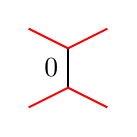
\begin{tikzpicture}[scale=1,baseline=(current bounding box.center)]
		\draw (.5,.25)--(.5,.75) node [pos=.5,left]{0};
		\draw [red, line width=0.25mm] (0,0) -- (.5,.25) -- (1,0);
		\draw [red, line width=0.25mm] (0,1) -- (.5,.75)--(1,1);
		\end{tikzpicture}
		=
		\alpha\ 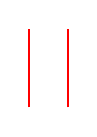
\begin{tikzpicture}[scale=1,baseline=(current bounding box.center)]
			\draw [red, line width=0.25mm] (0,0) -- (0,1);
			\draw [red, line width=0.25mm] (0.5,0) -- (0.5,1);
		\end{tikzpicture}
		+\beta\ 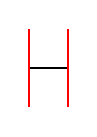
\begin{tikzpicture}[scale=1,baseline=(current bounding box.center)]
			\draw (0,0.5) -- (0.5,0.5);
			\draw [red, line width=0.25mm] (0,0) -- (0,1);
			\draw [red, line width=0.25mm] (0.5,0) -- (0.5,1);			
		\end{tikzpicture}\ .
	\end{equation*}
To compute $\alpha$ and $\beta$ above, in addition to the action on the spin chain, we will need the full set of $F$ symbols.

From the category $\Vec(\Z/2\Z)$, and the bimodule associators we have
\begin{align}
\left(F_{abc}^{a+b+c}\right)_{a+b,b+c}&=1&&\text{From Example~\ref{example:vecG}: $F$=+1}\\
\left(F_{ab*}^*\right)_{a+b,*}&=1&&\text{From Eqn.~\ref{eqn:L}: $L$=+1} \\
\left(F_{a*b}^*\right)_{*,*}&=(-1)^{ab}&&\text{From Eqn.~\ref{eqn:F1}} \\
\left(F_{*ab}^*\right)_{*,a+b}&=1&&\text{From Eqn.~\ref{eqn:R}: $R$=+1} \\
\left(F_{a**}^{a+b}\right)_{*,b}&=??\\
\left(F_{*a*}^b\right)_{*,*}&=??\\
\left(F_{**a}^{a+b}\right)_{b,*}&=??\\
\left(F_{***}^*\right)_{a,b}&=??,
\end{align}
	
We use the following normalization\cite{Bonderson,BSS08}:
	\begin{equation}
		\begin{tikzpicture}[scale=1.2,baseline=(current bounding box.center)]
			\draw (0,0) to node [left] {$a$} (0,1);
			\draw (0.5,0) to node [right] {$b$} (0.5,1);
		\end{tikzpicture}=\sum_c\ \sqrt{\frac{d_c}{d_a d_b}}\ 
		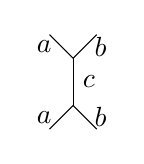
\begin{tikzpicture}[scale=1.2,baseline=(current bounding box.center)]
			\draw (0,0) to node [left] {$a$} (0.25,0.25);
			\draw (0.5,0) to node [right] {$b$} (0.25,0.25);
			\draw (0,1) to node [left] {$a$} (0.25,0.75);
			\draw (0.5,1) to node [right] {$b$} (0.25,0.75);
			\draw (0.25,0.25) to node [right] {$c$} (0.25,0.75);
		\end{tikzpicture}.
	\end{equation}
For the black strings in our diagrams, the sum has only one term and the coefficients are $d_0=1=d_1$, which yields the relation
	\begin{equation}
	\label{eq:completeness}
		\begin{tikzpicture}[scale=1.2,baseline=(current bounding box.center)]
			\draw (0,0) to node [left] {$a$} (0,1);
			\draw (0.5,0) to node [right] {$b$} (0.5,1);
		\end{tikzpicture}=
		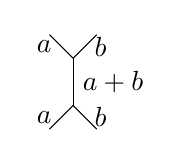
\begin{tikzpicture}[scale=1.2,baseline=(current bounding box.center)]
			\draw (0,0) to node [left] {$a$} (0.25,0.25);
			\draw (0.5,0) to node [right] {$b$} (0.25,0.25);
			\draw (0,1) to node [left] {$a$} (0.25,0.75);
			\draw (0.5,1) to node [right] {$b$} (0.25,0.75);
			\draw (0.25,0.25) to node [right] {$a+b$} (0.25,0.75);
		\end{tikzpicture}.
	\end{equation}
From the fusion rules, $d_*=\sqrt{2}$, so
\begin{equation}
\label{eq:completeness2}
\begin{tikzpicture}[scale=1.2,baseline=(current bounding box.center)]
\draw[red] (0,0) to (0,1);
\draw (0.5,0) to node [right] {$a$} (0.5,1);
\end{tikzpicture}=
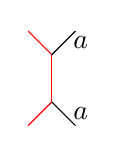
\begin{tikzpicture}[scale=1.2,baseline=(current bounding box.center)]
\draw[red] (0,0) to (0.25,0.25);
\draw (0.5,0) to node [right] {$a$} (0.25,0.25);
\draw[red] (0,1) to (0.25,0.75);
\draw (0.5,1) to node [right] {$a$} (0.25,0.75);
\draw[red] (0.25,0.25) to (0.25,0.75);
\end{tikzpicture}.
\end{equation}
The computation for $F_{**a}^{a+b}$ is particularly straightforward:
	\begin{align}
		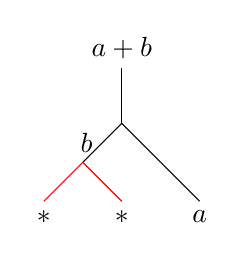
\begin{tikzpicture}[scale=0.7,baseline=(current bounding box.center)]
			\draw[] (0,0) -- (0,1) node[pos=1,above]{$a+b$};
			\draw[] (0,0) -- (-0.707107,-0.707107) node [pos=.5,left] {$b$};
			\draw[red] (-0.707107,-0.707107) -- (-1.41421,-1.41421);
			\draw[red] (-0.707107,-0.707107) -- (0,-1.41421);
			\draw (0,0) -- (0.707107,-0.707107);
			\draw (0.707107,-0.707107) -- (1.41421,-1.41421);
			\node at (-1.41421,-1.7) {$*$};
			\node at (0,-1.7) {$*$};
			\node at (1.41421,-1.7) {$a$};
		\end{tikzpicture}&=
		\frac{1}{4}\sum_{x,y}(-1)^{bx}
		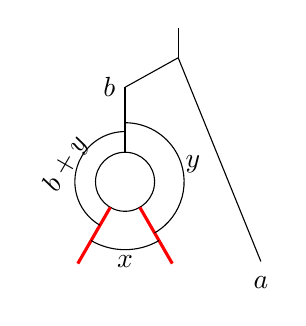
\begin{tikzpicture}[scale=.75,baseline=(current bounding box.center)]
			\draw (0,0) circle (0.5cm);
			\draw[red,line width=0.4mm]
			\foreach \a in {-60, -120} {
				(\a:0.5) -- (\a:1.6)
			};
			\draw[] (90:0.5) -- (90:1.6);
			\draw ([shift=(-60:1cm)]0,0) arc (-60:90:1cm);
			\draw ([shift=(-120:1.15cm)]0,0) arc (-120:-60:1.15cm);
			\draw ([shift=(240:0.85cm)]0,0) arc (240:90:0.85cm);
			\draw[] (0,1.6) -- (0.9,2.1) node[pos=0,left] {$b$};
			\draw[] (0.9,2.1) -- (0.9,2.6);
			\draw (0.9,2.1) -- (2.3,-1.35);
			\node[rotate=60] at (-1,0.3) {$b+y$};
			\node at (1.15,0.3) {$y$};
			\node at (2.3,-1.7) {$a$};
			\node at (0,-1.35) {$x$};
		\end{tikzpicture}
		=\frac{1}{4}\sum_{x,y}(-1)^{bx}
		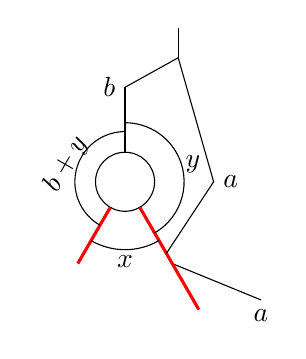
\begin{tikzpicture}[scale=.75,baseline=(current bounding box.center)]
		\draw (0,0) circle (0.5cm);
		\draw[red,line width=0.4mm]
		\foreach \a in {-60, -120} {
			(\a:0.5) -- (\a:1.6)
		};
		\draw[] (90:0.5) -- (90:1.6);
		\draw ([shift=(-60:1cm)]0,0) arc (-60:90:1cm);
		\draw ([shift=(-120:1.15cm)]0,0) arc (-120:-60:1.15cm);
		\draw ([shift=(240:0.85cm)]0,0) arc (240:90:0.85cm);
		\draw[] (0,1.6) -- (0.9,2.1) node[pos=0,left] {$b$};
		\draw[] (0.9,2.1) -- (0.9,2.6);
%		\draw (0.9,2.1) -- (2.3,-1.35);
		\draw (-60:1.6) -- (2.3,-2) node[pos=1,below] {$a$};
		\draw (-60:1.4) --(1.5,0) node[right]{$a$} -- (0.9,2.1);
		\node[rotate=60] at (-1,0.3) {$b+y$};
		\node at (1.15,0.3) {$y$};
%		\node at (2.3,-1.7) {$a$};
		\node at (0,-1.35) {$x$};
		\draw[red,line width=0.4mm] (-60:1.6)--(-60:2.5);
		\end{tikzpicture}
		\\
		&=\frac{1}{4}\sum_{x,y}(-1)^{(a+b)x}
		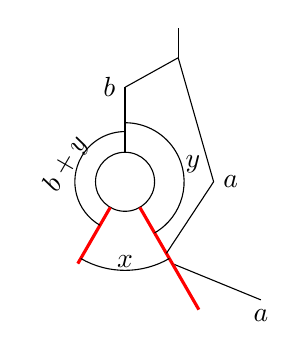
\begin{tikzpicture}[scale=.75,baseline=(current bounding box.center)]
		\draw (0,0) circle (0.5cm);
		\draw[red,line width=0.4mm]
		\foreach \a in {-60, -120} {
			(\a:0.5) -- (\a:1.6)
		};
		\draw[] (90:0.5) -- (90:1.6);
		\draw ([shift=(-60:1cm)]0,0) arc (-60:90:1cm);
		\draw ([shift=(-120:1.5cm)]0,0) arc (-120:-60:1.5cm);
		\draw ([shift=(240:0.85cm)]0,0) arc (240:90:0.85cm);
		\draw[] (0,1.6) -- (0.9,2.1) node[pos=0,left] {$b$};
		\draw[] (0.9,2.1) -- (0.9,2.6);
		%		\draw (0.9,2.1) -- (2.3,-1.35);
		\draw (-60:1.6) -- (2.3,-2) node[pos=1,below] {$a$};
		\draw (-60:1.4) --(1.5,0) node[right]{$a$} -- (0.9,2.1);
		\node[rotate=60] at (-1,0.3) {$b+y$};
		\node at (1.15,0.3) {$y$};
		%		\node at (2.3,-1.7) {$a$};
		\node at (0,-1.35) {$x$};
		\draw[red,line width=0.4mm] (-60:1.6)--(-60:2.5);
		\end{tikzpicture}
		=\frac{1}{4}\sum_{x,y}(-1)^{(a+b)x}
		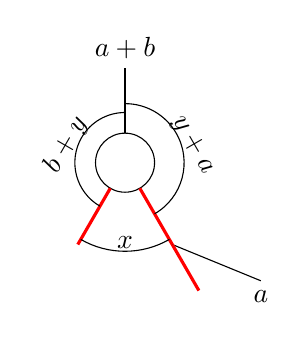
\begin{tikzpicture}[scale=.75,baseline=(current bounding box.center)]
		\draw (0,0) circle (0.5cm);
		\draw[red,line width=0.4mm]
		\foreach \a in {-60, -120} {
			(\a:0.5) -- (\a:1.6)
		};
		\draw[] (90:0.5) -- (90:1.6) node[pos=1,above]{$a+b$};
		\draw ([shift=(-60:1cm)]0,0) arc (-60:90:1cm);
		\draw ([shift=(-120:1.5cm)]0,0) arc (-120:-60:1.5cm);
		\draw ([shift=(240:0.85cm)]0,0) arc (240:90:0.85cm);
%		\draw[] (0,1.6) -- (0.9,2.1) ;
%		\draw[] (0.9,2.1) -- (0.9,2.6);
		%		\draw (0.9,2.1) -- (2.3,-1.35);
		\draw (-60:1.6) -- (2.3,-2) node[pos=1,below] {$a$};
%		\draw (-60:1.4) --(1.5,0) node[right]{$a$} -- (0.9,2.1);
		\node[rotate=60] at (-1,0.3) {$b+y$};
		\node[rotate=-60] at (1.15,0.3) {$y+a$};
		%		\node at (2.3,-1.7) {$a$};
		\node at (0,-1.35) {$x$};
		\draw[red,line width=0.4mm] (-60:1.6)--(-60:2.5);
		\end{tikzpicture}\\
		&=\frac{1}{4}\sum_{x,y^\prime}(-1)^{(a+b)x}
		\begin{tikzpicture}[scale=.75,baseline=(current bounding box.center)]
		\draw (0,0) circle (0.5cm);
		\draw[red,line width=0.4mm]
		\foreach \a in {-60, -120} {
			(\a:0.5) -- (\a:1.6)
		};
		\draw[] (90:0.5) -- (90:1.6) node[pos=1,above]{$a+b$};
		\draw ([shift=(-60:1cm)]0,0) arc (-60:90:1cm);
		\draw ([shift=(-120:1.5cm)]0,0) arc (-120:-60:1.5cm);
		\draw ([shift=(240:0.85cm)]0,0) arc (240:90:0.85cm);
		\draw (-60:1.6) -- (2.3,-2) node[pos=1,below] {$a$};
		\node[rotate=60] at (-1,0.3) {$a+b+y^\prime$};
		\node at (1.15,0.3) {$y^\prime$};
		\node at (0,-1.35) {$x$};
		\draw[red,line width=0.4mm] (-60:1.6)--(-60:2.5);
		\end{tikzpicture}
		=\begin{tikzpicture}[xscale=-1,scale=0.7,baseline=(current bounding box.center)]
		\draw[] (0,0) -- (0,1) node[pos=1,above]{$a+b$};
		\draw[red] (0,0) -- (-0.707107,-0.707107);
		\draw[] (-0.707107,-0.707107) -- (-1.41421,-1.41421);
		\draw[red] (-0.707107,-0.707107) -- (0,-1.41421);
		\draw[red] (0,0) -- (0.707107,-0.707107);
		\draw[red] (0.707107,-0.707107) -- (1.41421,-1.41421);
		\node at (-1.41421,-1.7) {$a$};
		\node at (0,-1.7) {$*$};
		\node at (1.41421,-1.7) {$*$};
		\end{tikzpicture}
	\end{align}
so it follows that 
	\begin{equation}
		\left(F_{**a}^{a+b}\right)_{b,*}=1.
	\end{equation}
The computation of $\left(F_{a**}^{a+b}\right)_{*,b}=1$ is identical. A similar computation yields $\left(F_{*a*}^{b}\right)_{*,*}=(-1)^{ab}$.


\subsection*{Step 6: Check if $F$-symbols obey the pentagon equation} To check whether the maps that we have just defined obey the pentagon equation, we need the full set of $F$-symbols. This means that, in addition to the vertex we have just computed, we also need to compute the vertex
	\begin{figure}[H]
		\begin{tikzpicture}
			\draw[red,line width=0.4mm] (0,0) -- (1.5,0);
			\draw (0.75,0) -- (0.75,1);
		\end{tikzpicture}
	\end{figure}
\noindent
Doing the same steps as above yields
	\begin{equation*}
		\begin{tikzpicture}[scale=1,baseline=(current bounding box.center)]
			\draw[red,line width=0.4mm] (0,0) -- (1.5,0);
			\draw (0.75,0) to node[near end, right] {$\mu$} (0.75,1);
		\end{tikzpicture}=\frac{1}{4}\sum_{x,y}(-1)^{\mu y}
		\begin{tikzpicture}[scale=1,baseline=(current bounding box.center)]
			\draw (0,0) circle (0.5cm);
			\draw[red,line width=0.4mm]
			\foreach \a in {-60, -120} {
				(\a:0.5) -- (\a:1.6)
			};
			\draw (90:0.5) to node[near end, right] {$\mu$} (90:1.6);
			\draw ([shift=(-60:1cm)]0,0) arc (-60:90:1cm);
			\draw ([shift=(-120:1.15cm)]0,0) arc (-120:-60:1.15cm);
			\draw ([shift=(240:0.85cm)]0,0) arc (240:90:0.85cm);
			\node at (0.2,-0.2) {$0$};
			\node at (-0.2,-0.2) {$0$};
			\node at (-1,0.3) {$x$};
			\node at (1.15,0.3) {$x$};
			\node at (0,-1.35) {$y$};
		\end{tikzpicture}.
	\end{equation*}
Using all the vertices we have defined enables us to calculate the whole set of $F$-symbols:
	\begin{align*}
		\left(F_{abc}^{a+b+c}\right)_{a+b,b+c}&=1\\
		\left(F_{ab*}^*\right)_{a+b,*}&=1\\
		\left(F_{a*b}^*\right)_{*,*}&=(-1)^{ab}\\
		\left(F_{*ab}^*\right)_{*,a+b}&=1\\
		\left(F_{a**}^{a+b}\right)_{*,b}&=1\\
		\left(F_{*a*}^b\right)_{*,*}&=(-1)^{ab}\\
		\left(F_{**a}^{a+b}\right)_{b,*}&=1\\
		\left(F_{***}^*\right)_{a,b}&=\frac{1}{\sqrt{2}}(-1)^{ab},
	\end{align*}
which happen to be the $F$-symbols for the Ising category. 

We now want to build a chain out of $\Vec(\Z/2\Z)$ and the bimodule $F_1$ in the following way: consider the chain
	\begin{figure}[H]
		\begin{tikzpicture}
			\draw[blue,line width=0.4mm] (-0.25,0) -- (8.25,0);
			\draw[red,line width=0.4mm] (0.5,0) -- (0.5,1);
			\draw[red,line width=0.4mm] (1.5,0) -- (1.5,1);
			\draw[red,line width=0.4mm] (2.5,0) -- (2.5,1);
			\draw[red,line width=0.4mm] (3.5,0) -- (3.5,1);
			\draw[red,line width=0.4mm] (4.5,0) -- (4.5,1);
			\draw[red,line width=0.4mm] (5.5,0) -- (5.5,1);
			\draw[red,line width=0.4mm] (6.5,0) -- (6.5,1);
			\draw[red,line width=0.4mm] (7.5,0) -- (7.5,1);
		\end{tikzpicture}
	\end{figure}
\noindent
where
	\begin{equation}
		\begin{tikzpicture}[scale=1,baseline=(current bounding box.center)]
			\draw[blue,line width=0.4mm] (0,0) -- (1,0);
		\end{tikzpicture}=
		\begin{tikzpicture}[scale=1,baseline=(current bounding box.center)]
			\draw[black,line width=0.4mm] (0,0) -- (1,0);
		\end{tikzpicture}\oplus
		\begin{tikzpicture}[scale=1,baseline=(current bounding box.center)]
			\draw[red,line width=0.4mm] (0,0) -- (1,0);
		\end{tikzpicture},
	\end{equation}
which means that it is either an object from the category ($0$ or $1$) or an object from the bimodule (which can only be $*$), i.e., $\mathbb{C}^2\oplus\mathbb{C}\cong\mathbb{C}^3$. Valid configurations then look like
	\begin{figure}[H]
		\begin{tikzpicture}
			\draw[black,line width=0.4mm] (-0.25,0) to node [below] {$\mathbb{C}^2$} (0.5,0);
			\draw[red,line width=0.4mm] (0.5,0) -- (0.5,1);
			\draw[red,line width=0.4mm] (0.5,0) -- (1.5,0);
			\draw[red,line width=0.4mm] (1.5,0) -- (1.5,1);
			\draw[black,line width=0.4mm] (1.5,0) to node [below] {$\mathbb{C}^2$} (2.5,0);
			\draw[red,line width=0.4mm] (2.5,0) -- (2.5,1);
			\draw[red,line width=0.4mm] (2.5,0) -- (3.5,0);
			\draw[red,line width=0.4mm] (3.5,0) -- (3.5,1);
			\draw[black,line width=0.4mm] (3.5,0) to node [below] {$\mathbb{C}^2$} (4.5,0);
			\draw[red,line width=0.4mm] (4.5,0) -- (4.5,1);
			\draw[red,line width=0.4mm] (4.5,0) -- (5.5,0);
			\draw[red,line width=0.4mm] (5.5,0) -- (5.5,1);
			\draw[black,line width=0.4mm] (5.5,0) to node [below] {$\mathbb{C}^2$} (6.5,0);
			\draw[red,line width=0.4mm] (6.5,0) -- (6.5,1);
			\draw[red,line width=0.4mm] (6.5,0) -- (7.5,0);
			\draw[red,line width=0.4mm] (7.5,0) -- (7.5,1);
			\draw[black,line width=0.4mm] (7.5,0) to node [below] {$\mathbb{C}^2$} (8.25,0);
		\end{tikzpicture}
	\end{figure}
\noindent
so we have a non-trivial Hilbert space. We will now construct a Hamiltonian for this chain that is similar to the golden chain Hamiltonian in \cite{Feiguin2007}, where a chain model for the Fibonacci category was constructed which energetically favoured fusing to the vacuum. For our chain model, this means that it is energetically favoured to fuse to the $0$ object of $\Vec(\Z/2\Z)$. Hence, the Hamiltonian is of the form
	\begin{equation}
		H=-\sum \frac{1}{\sqrt{2}}
		\begin{tikzpicture}[scale=0.5,baseline=(current bounding box.center)]
			\draw[red,line width=0.4mm] (0,0) -- (-0.7,0.9);
			\draw[red,line width=0.4mm] (0,0) -- (0.7,0.9);
			\draw (0,0) to node[right] {$0$} (0,-1);
			\draw[red,line width=0.4mm] (0,-1) -- (-0.7,-1.9);
			\draw[red,line width=0.4mm] (0,-1) -- (0.7,-1.9);
%			\node at (0.8,1.1) {$*$};
%			\node at (-0.8,1.1) {$*$};
%			\node at (0.8,-2.1) {$*$};
%			\node at (-0.8,-2.1) {$*$};
		\end{tikzpicture},
	\end{equation}
where the sum goes over all sites of the chain. To be able to act on the chain with this Hamiltonian, we first need to change the basis using the identity
	\begin{equation}
		\begin{tikzpicture}[scale=0.5,baseline=(current bounding box.center)]
			\draw (0,0) -- (-0.7,0.9);
			\draw (0,0) -- (0.7,0.9);
			\draw (0,0) to node[right] {$e$} (0,-1);
			\draw (0,-1) -- (-0.7,-1.9);
			\draw (0,-1) -- (0.7,-1.9);
			\node at (0.8,1.2) {$b$};
			\node at (-0.8,1.2) {$a$};
			\node at (0.8,-2.2) {$d$};
			\node at (-0.8,-2.2) {$c$};
		\end{tikzpicture}=\sum_f\left(F_d^{abc}\right)_{ef}
		\begin{tikzpicture}[scale=0.5,baseline=(current bounding box.center)]
			\draw (0,0) -- (-0.9,0.7);
			\draw (0,0) -- (-0.9,-0.7);
			\draw (0,0) to node[above] {$f$} (1,0);
			\draw (1,0) -- (1.9,0.7);
			\draw (1,0) -- (1.9,-0.7);
			\node at (-1.2,0.8) {$a$};
			\node at (-1.2,-0.8) {$c$};
			\node at (2.2,0.8) {$b$};
			\node at (2.2,-0.8) {$d$};
		\end{tikzpicture}
	\end{equation}
which yields
	\begin{align}
		H&=-\sum \frac{1}{\sqrt{2}}\left(\left(F_*^{***}\right)_{00}
		\begin{tikzpicture}[scale=0.5,baseline=(current bounding box.center)]
			\draw[red,line width=0.4mm] (0,0) -- (0,2);
			\draw[red,line width=0.4mm] (1.5,0) -- (1.5,2);
		\end{tikzpicture}+\left(F_*^{***}\right)_{01}
		\begin{tikzpicture}[scale=0.5,baseline=(current bounding box.center)]
			\draw[red,line width=0.4mm] (0,0) -- (0,2);
			\draw (0,1) to node[above] {$1$} (1.5,1);
			\draw[red,line width=0.4mm] (1.5,0) -- (1.5,2);
		\end{tikzpicture}\ \right)\\
		&=-\sum\frac{1}{\sqrt{2}}\left(\ 
		\begin{tikzpicture}[scale=0.5,baseline=(current bounding box.center)]
			\draw[red,line width=0.4mm] (0,0) -- (0,2);
			\draw[red,line width=0.4mm] (1.5,0) -- (1.5,2);
		\end{tikzpicture}+
		\begin{tikzpicture}[scale=0.5,baseline=(current bounding box.center)]
			\draw[red,line width=0.4mm] (0,0) -- (0,2);
			\draw (0,1) to node[above] {$1$} (1.5,1);
			\draw[red,line width=0.4mm] (1.5,0) -- (1.5,2);
		\end{tikzpicture}\ \right),
	\end{align}
where we have used the $F$-symbols we have computed above. Now we study how this Hamiltonian acts on the valid local configurations
	\begin{figure}[H]
		\begin{tikzpicture}[scale=1,baseline=(current bounding box.center)]
			\draw (-0.5,0) -- (0,0);
			\draw [red, line width=0.25mm] (0,0) -- (1,0);
			\draw (1,0) -- (1.5,0);
			\draw [red, line width=0.25mm] (0,0) -- (0,1);
			\draw [red, line width=0.25mm] (1,0) -- (1,1);
			\node at (-0.7,0) {$a$};
			\node at (1.7,0) {$b$};
		\end{tikzpicture} \hspace{20pt}
		\begin{tikzpicture}[scale=1,baseline=(current bounding box.center)]
			\draw [red, line width=0.25mm] (-0.5,0) -- (0,0);
			\draw (0,0) -- (1,0);
			\draw [red, line width=0.25mm] (1,0) -- (1.5,0);
			\draw [red, line width=0.25mm] (0,0) -- (0,1);
			\draw [red, line width=0.25mm] (1,0) -- (1,1);
			\node at (-0.7,0) {$a$};
			\node at (1.7,0) {$b$};
		\end{tikzpicture}
	\end{figure}
\noindent
The first term of the Hamiltonian leaves the configurations invariant, while the second term acts in the following way:
	\begin{align}
		\begin{tikzpicture}[scale=1,baseline=(current bounding box.center)]
			\draw (-0.5,0) -- (0,0);
			\draw [red, line width=0.25mm] (0,0) -- (1,0);
			\draw (1,0) -- (1.5,0);
			\draw [red, line width=0.25mm] (0,0) -- (0,1);
			\draw (0,0.5) to node[above] {$1$} (1,0.5);
			\draw [red, line width=0.25mm] (1,0) -- (1,1);
			\node at (-0.7,0) {$a$};
			\node at (1.7,0) {$b$};
		\end{tikzpicture}&=
		\begin{tikzpicture}[scale=1,baseline=(current bounding box.center)]
			\draw (-0.5,0) -- (0,0);
			\draw [red, line width=0.25mm] (0,0) -- (1,0);
			\draw (1,0) -- (1.5,0);
			\draw [red, line width=0.25mm] (0,0) -- (0,1);
			\draw [red, line width=0.25mm] (1,0) -- (1,1);
			\node at (-0.7,0) {$a$};
			\node at (1.7,0) {$b$};
			\draw (0,0.5) to[bend left] node[above] {$1$} (0.4,0);
			\draw (1,0.5) to[bend right] node[above] {$1$} (0.6,0);
		\end{tikzpicture}=(-1)^{a+b}
		\begin{tikzpicture}[scale=1,baseline=(current bounding box.center)]
			\draw (-0.5,0) -- (0,0);
			\draw [red, line width=0.25mm] (0,0) -- (1,0);
			\draw (1,0) -- (1.5,0);
			\draw [red, line width=0.25mm] (0,0) -- (0,1);
			\draw [red, line width=0.25mm] (1,0) -- (1,1);
			\node at (-0.7,0) {$a$};
			\node at (1.7,0) {$b$};
		\end{tikzpicture}\equiv Z_a\otimes Z_b\\
		\begin{tikzpicture}[scale=1,baseline=(current bounding box.center)]
			\draw [red, line width=0.25mm] (-0.5,0) -- (0,0);
			\draw (0,0) to node[below] {$a$} (1,0);
			\draw [red, line width=0.25mm] (1,0) -- (1.5,0);
			\draw [red, line width=0.25mm] (0,0) -- (0,1);
			\draw [red, line width=0.25mm] (1,0) -- (1,1);
			\draw (0,0.5) to node[above] {$1$} (1,0.5);
		\end{tikzpicture}&=
		\begin{tikzpicture}[scale=1,baseline=(current bounding box.center)]
			\draw [red, line width=0.25mm] (-0.5,0) -- (0,0);
			\draw (0,0) to node[below] {$a+1$} (1,0);
			\draw [red, line width=0.25mm] (1,0) -- (1.5,0);
			\draw [red, line width=0.25mm] (0,0) -- (0,1);
			\draw [red, line width=0.25mm] (1,0) -- (1,1);
		\end{tikzpicture}\equiv X_a
	\end{align}
Hence, in general the local Hamiltonian $h_i$ acts like
	\begin{align*}
		h_i \left(\begin{tikzpicture}[scale=1,baseline=(current bounding box.center)]
		\draw [blue, line width=0.25mm] (-0.5,0) to node[below, near start] {$x_{i-1}$} (0,0);
		\draw [blue, line width=0.25mm] (0,0) to node[below] {$x_i$} (1,0);
		\draw [blue, line width=0.25mm] (1,0) to node[below, near end] {$x_{i+1}$} (1.5,0);
		\draw [red, line width=0.25mm] (0,0) -- (0,1);
		\draw [red, line width=0.25mm] (1,0) -- (1,1);
		\end{tikzpicture}\right)=&\left(\left(Z_{x_{i-1}}\oplus 0\right)\otimes\left(0\oplus\lvert*\rangle_{x_i}\langle*\rvert\right)\otimes\left(Z_{x_{i+1}}\oplus 0\right)\right.\\&+\left.\left(0\oplus\lvert*\rangle_{x_{i-1}}\langle*\rvert\right)\otimes\left(Z_{x_i}\oplus 0\right)\otimes\left(0\oplus \lvert *\rangle_{x_{i-1}}\langle *\rvert\right)\right)\left(\begin{tikzpicture}[scale=1,baseline=(current bounding box.center)]
		\draw [blue, line width=0.25mm] (-0.5,0) to node[below, near start] {$x_{i-1}$} (0,0);
		\draw [blue, line width=0.25mm] (0,0) to node[below] {$x_i$} (1,0);
		\draw [blue, line width=0.25mm] (1,0) to node[below, near end] {$x_{i+1}$} (1.5,0);
		\draw [red, line width=0.25mm] (0,0) -- (0,1);
		\draw [red, line width=0.25mm] (1,0) -- (1,1);
		\end{tikzpicture}\right).
	\end{align*}
Fixing boundary conditions to $*$ freezes out half of the valid configurations, which results in the Ising model.